\IEEEPARstart{T}{he} second assignment is going to utilize results from the first assignment and
thus the dataset has to be the same: "CIFAR-10".
\begin{itemize}
  \item \url{https://www.cs.toronto.edu/~kriz/cifar.html}
\end{itemize}

It consists of 60000 32x32 color images which belong to one of the 10 available classes. There are
6000 images per class, 5000 training images and 1000 test images. The data is available in 6 
batches of 10000 images each.
\begin{itemize}
  \item five training batches (50,000 or 5000 images from each class)
  \item one test batch (10,000 or 1000 images from each class)
\end{itemize}
Since the training batches' images are chosen randomly, each batch individually may contain more 
images from one class than another but, cumulatively, the number of images from each class is 
equal. Here is an example of the dataset's structure:

\begin{figure}[H]
  \centering
  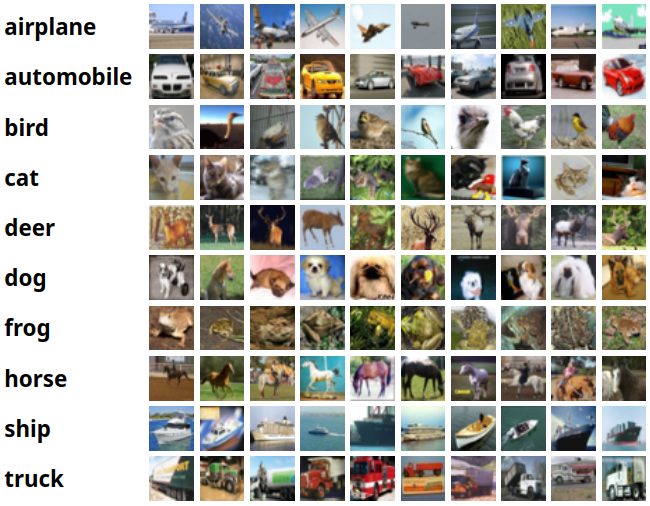
\includegraphics[width=2.5in]{media/cifar10_example.png}
  \caption{The CIFAR-10 dataset.}
  \label{CIFAR example}
\end{figure}